\textcolor{blue}{
	\subsection{Illustration on a simplified brain imaging dataset}
	\label{sec:proof_of_concept}
\refnum{\#5, \#6, \#8}
	In this section we describe a simple experiment where we use MT-MCVAE to model the joint relationship between
	magnetic resonance imaging (MRI) and fluorodeoxyglucose positron emission tomography (FDG-PET) images when there are missing data at training time.
	The trained model will be then applied on test data
	to the cross-modality reconstruction problem (MRI to FDG-PET and \textit{vice versa}).
%	
	Data comes from the `Adni2'
	\footnote{
	\href{http://adni.loni.usc.edu}{adni.loni.usc.edu}.
	The ADNI was launched in 2003 as a public-private partnership, led by Principal Investigator Michael W. Weiner, MD. For up-to-date information, see \href{www.adni-info.org}{www.adni-info.org}.
	}
	dataset (see details in \S~\ref{ssec:datasets}, \tabref{table:datasets}), from which we took the MRI and FDG-PET brain imaging modalities.
	In what follows, each one of this two modalities corresponds to a specific data view.
	For each subject ($n=424$, with both MRI and FDG-PET) we extracted $3$ brain slices for each one of the sagittal, coronal, and axial plane.
	The resulting $3816$ slices were randomly allocated to a training and testing set with respectively sizes of $3500$ and $316$ samples.
	We downsampled the slices to dimension $28 \times 28$ ($784$ pixels).
	%
	To simulate a datasets with missing views, we controlled for the fraction of observations with complete views ($f$) in the training set:
	this procedure is depicted in \figref{fig:nimg_scheme} where we show an example of training dataset created with $f=1/3$.
	%
	For our experiments we took all the $3500$ training images and we randomly removed MRI and FDG-PET views to obtain different training sets for which $f \in \{0, 0.25, 0.5, 0.75, 1\}$.
	In the case $f = 0$, from each subjects we kept only its MRI or FDG-PET slices, representing the limit case where no direct relationship between views is observable.
	In the limit case $f = 1$, all MRI and FDG-PET are paired, representing the ideal case of no missing views, that is the working case of the MCVAE \citep{Antelmi2019}.
	We adopted a deep architecture with $4$ layers for both encoders and decoders, having ReLU activation functions and layer dimensions of $784-1024-1024-16$ in the encoding and $16-1024-1024-784$ in the decoding path,
	an architecture inspired from those used by \cite{dcca1} and \cite{dcca2} for a similar task on the MNIST dataset \citep{mnist}.
	We adopted a Gaussian likelihood for the decoders, with independent diagonal covariance parameters, and
\refnum{\#9}
	we trained our model with mini-batches of size $500$ for $3000$ epochs, after setting up the Adam optimizer with a learning rate of 0.001.
	Training was repeated $5$ times, by changing the initialization random seed of the model parameters.
%	
	\begin{figure}[!h]
\centering
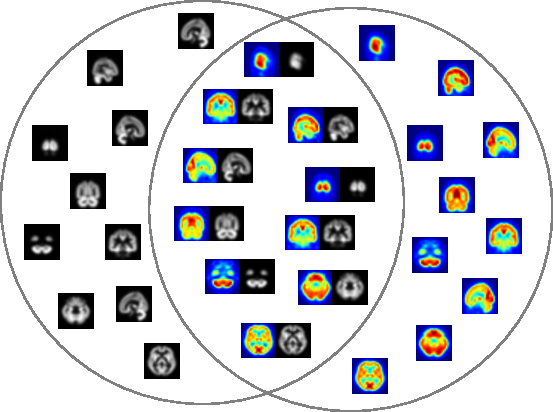
\includegraphics[width=0.8\columnwidth]{./tex/fig/nimg_scheme.pdf}
\caption{
	Pictorial example of training imaging dataset with two views, named \textit{left} and \textit{right} views.
	In this case we have 30 independent observations:
	$10$ with left-views only; $10$ with right-views only; $10$ with complete views.
	The fraction f of observations with complete views is:
	$f = 1/3$.
}
\label{fig:nimg_scheme}
\end{figure}
%
\begin{figure}[!h]
\centering
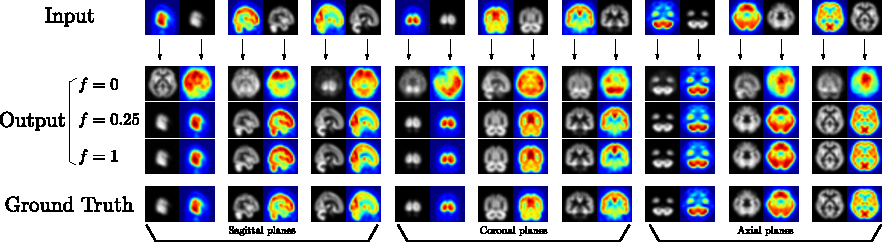
\includegraphics[width=\columnwidth]{./tex/fig/nimg_test.pdf}
\caption{
	Reconstruction of test-set digits when models are trained with an increasing fraction ($f$) of observations with complete-views.
	The left side of each digit is inferred from the input right side and \textit{vice versa}.
}
\label{fig:nimg_test}
\end{figure}

	\begin{table}[h]
\centering
\caption{
	Mean squared error (MSE) and negative log-likelihood (NLL) - the lower the better -  measured as mean (st.dev) on the reconstructed brain images of the test-set.
	The MRI were used to infer the FDG slices in the same subject, and \textit{vice versa}.
	Results stratified by $f$, the fraction of observations with no missing views in the training set.
	Notice the immediate drop in the error metrics as soon as $f$ increases.
}
\label{tab:nimg}
\resizebox{\columnwidth}{!}{
	\begin{tabular}{llllll}
	\toprule
	f                &             0.00 &           0.25 &           0.50 &           0.75 &           1.00 \\
	\midrule
	MSE             &     40.72 (4.31)  &  1.77 (0.04)  &  1.63 (0.06)  &  1.54 (0.03)  &  1.51 (0.03) \\
	NLL             &    96.44 (10.33)  &  0.53 (0.09)  &  0.16 (0.12)  &  -0.07 (0.07)  &  -2.63 (0.03)  \\
	\bottomrule
	\end{tabular}
}
\end{table}

	In \tabref{tab:nimg} we show the Mean Squared Error (MSE) and Negative Log-Likelihood (NLL) when predicting MRI from the FDG-PET slices and \textit{vice versa} in the testing set.
	We notice the immediate drop in the error metrics as soon as the parameter $f$ increases,
	which means that as the model is fed with an increasing proportion of multi-view data points in the training set,
	its predictions on the testing set become more precise.
}
	%
	% In \figref{fig:nimg_test} is possible to visually inspect these predictions.
